\label{ch:AnalyzingGraphs}

\begin{jointwork}
	In this chapter, we will put the tools and workflows described in the previous sections to the use. We will train two different Reinforcement-Learning Agents on different marketplaces, and then monitor them using all of the tools at our disposal, highlighting where each tool is most useful, and what could be improved.
\end{jointwork}

\section*{Setting up the experiments}

\subsection*{SAC-Duopoly}

We will first be conducting two different experiments: For one experiment, we will train a Reinforcement-Learning Agent using the SAC-algorithm (see \nameref{item:StableBaselines}) on a Duopoly marketplace with rebuy prices. The agent will be trained against a Rule-Based agent, more specifically the \emph{RuleBasedCERebuyAgentStorageMinimizer}, as presented in \nameref{subsec:DataDrivenModels}. The concrete configurations can be found in \Cref{fig:SACDuopolyConfigEnvironment} and \Cref{fig:SACDuopolyConfigMarket}. We will refer to this experiment as the \emph{SAC-Duopoly}.

\subsection*{PPO-Oligopoly}

For the second experiment, we will be training a different Reinforcement-Learning agent on a more complex market with more participants: A PPO-agent (\nameref{item:StableBaselines}) will be trained on an Oligopoly-Scenario, again with rebuy prices enabled. Three different Rule-Based agents will compete against the PPO-Agent on the same market:

\begin{enumerate}
	\item A \emph{FixedPriceAgent}, which will always set the following three prices:
	      \begin{itemize}
		      \item New price: 7
		      \item Refurbished price: 4
		      \item Rebuy price: 2
	      \end{itemize}
	      It should be noted that the configured maximum possible price is 10, which can also be configured using the configuration files. Depending on this maximum price, the prices set by \emph{FixedPriceAgents} must be adjusted to allow them to realistically compete in the market.
	\item The second agent is a \emph{RuleBasedCERebuyAgentCompetitive}, a more complicated and sophisticated version of the simple \emph{RuleBasedCEAgent}, which was introduced in \nameref{subsec:InventoryBasedModels}. The competitive version used for this experiment combines features of both the basic \emph{RuleBasedCEAgent} and the \emph{RuleBasedCERebuyAgentStorageMinimizer}. It's policy implementation can be found in \todo{Insert code snippet in Appendix}xyz.
	\item For the third competitor, we will again be using the \emph{RuleBasedCERebuyAgentStorageMinimizer}.
\end{enumerate}

This experiment will be referred to as the \emph{PPO-Oligopoly}.

\section*{Experiment results}

A commonly asked question when deciding on the quality of a Reinforcement-Learning Agent is their \emph{stability}\todo{cite?}. If an algorithm is stable, the trained agent will produce similar results over multiple training sessions, on the condition that the parameters do not differ. Not only the rewards achieved at the end of the training will be very similar, but also the amount of episodes needed to reach certain thresholds. In the case of the SAC-Duopoly experiment, we ran the same configuration three four times: For the first three times we used the exact same parameters, in the fourth experiment we tripled the amount of training episodes, meaning that the SAC-Agent had more time to alter its policy. \Cref{fig:SACDuopolyProfits} shows the results of these three training sessions, created using the \nameref{subsec:LiveMonitoring} tool, which runs directly after training has concluded, visualizing the data collected during the training process.

\begin{figure}[ht]
	\begin{subfigure}{\textwidth}
		\centering
		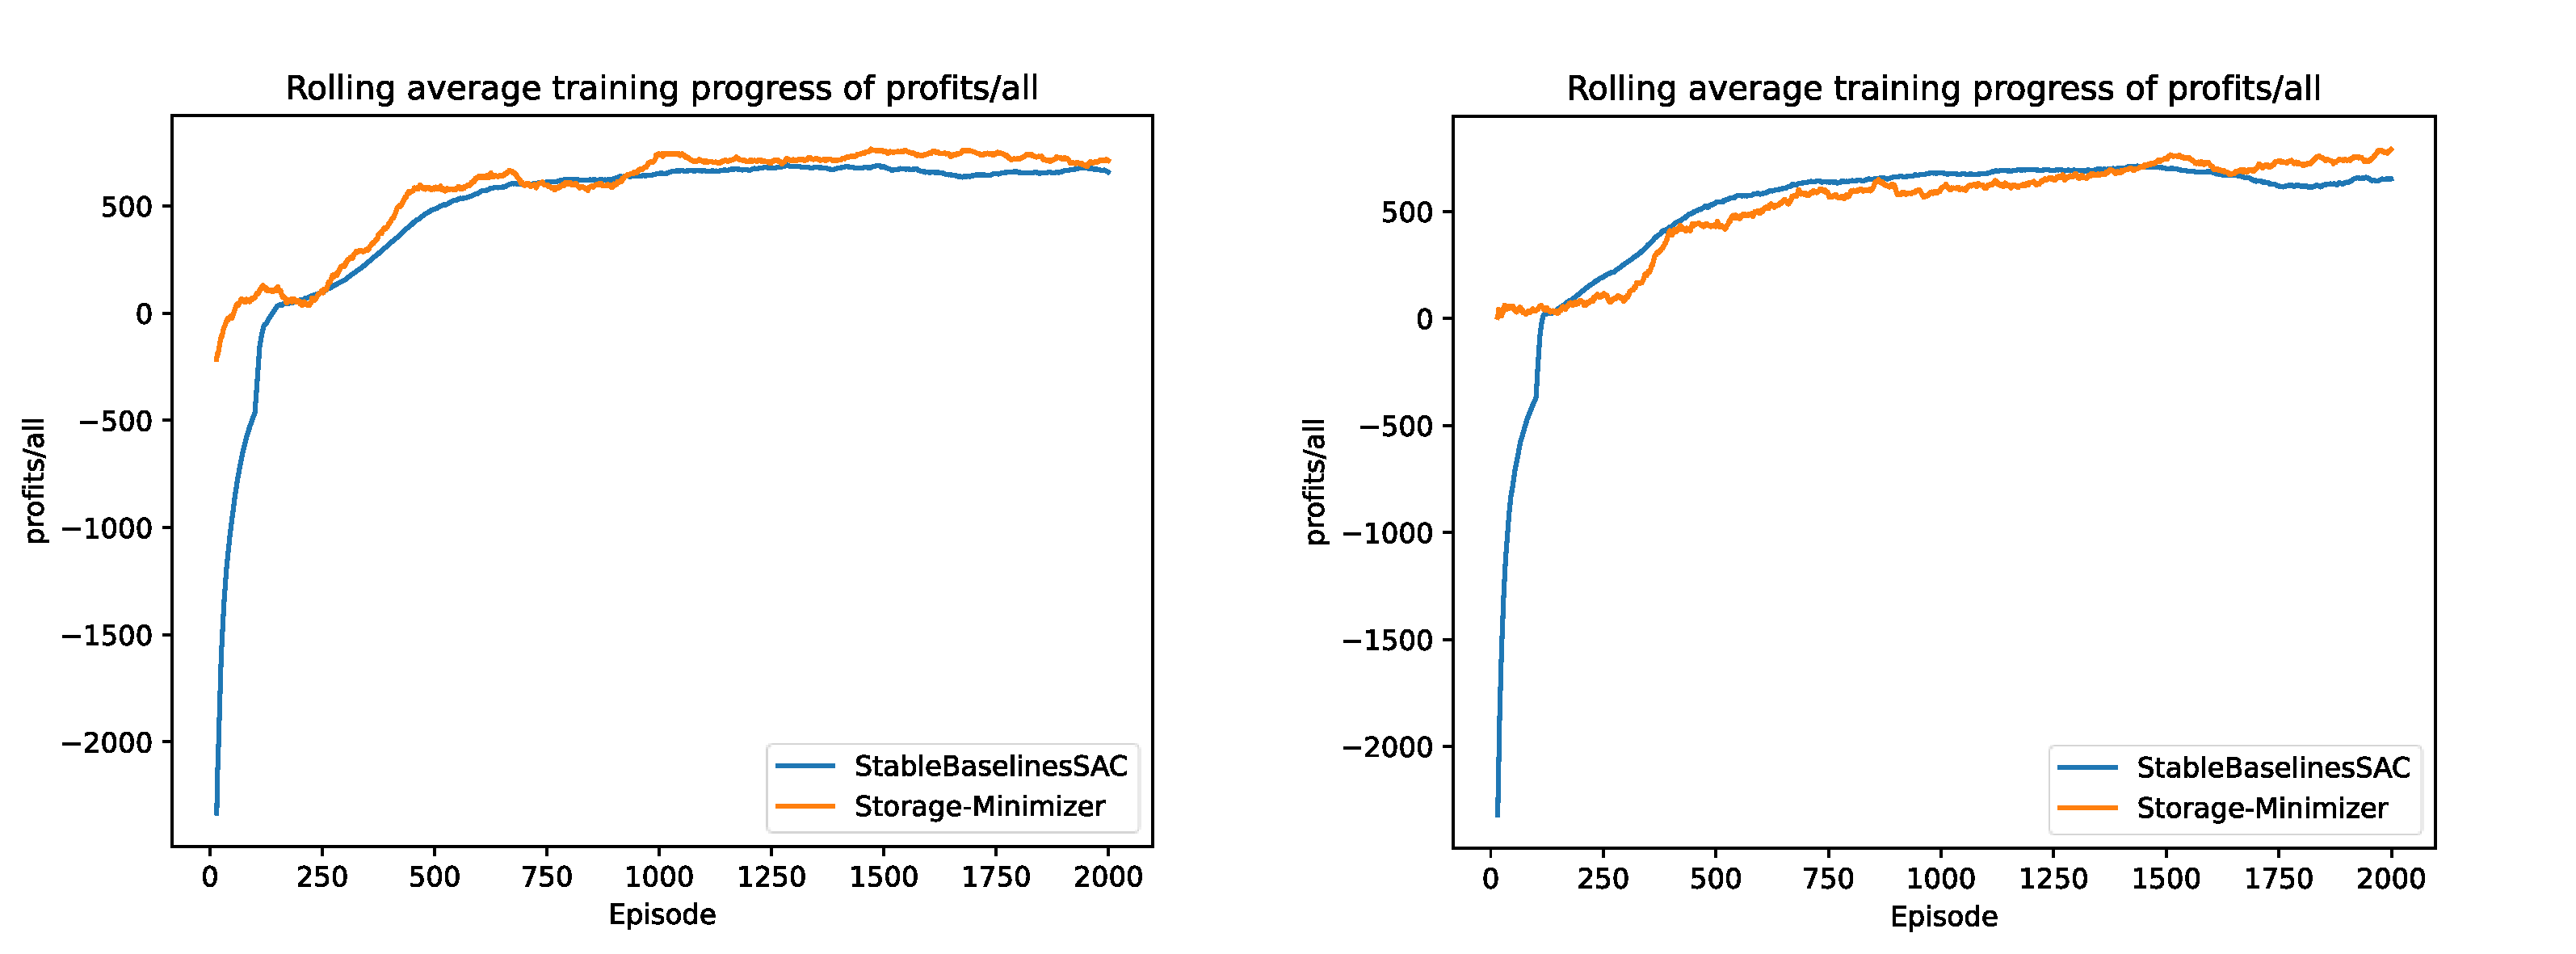
\includegraphics[width = \textwidth]{images/experiments/SACDuopoly/SACDuopolyProfits1_2.pdf}\\[1 ex]
	\end{subfigure}
	\begin{subfigure}{\textwidth}
		\centering
		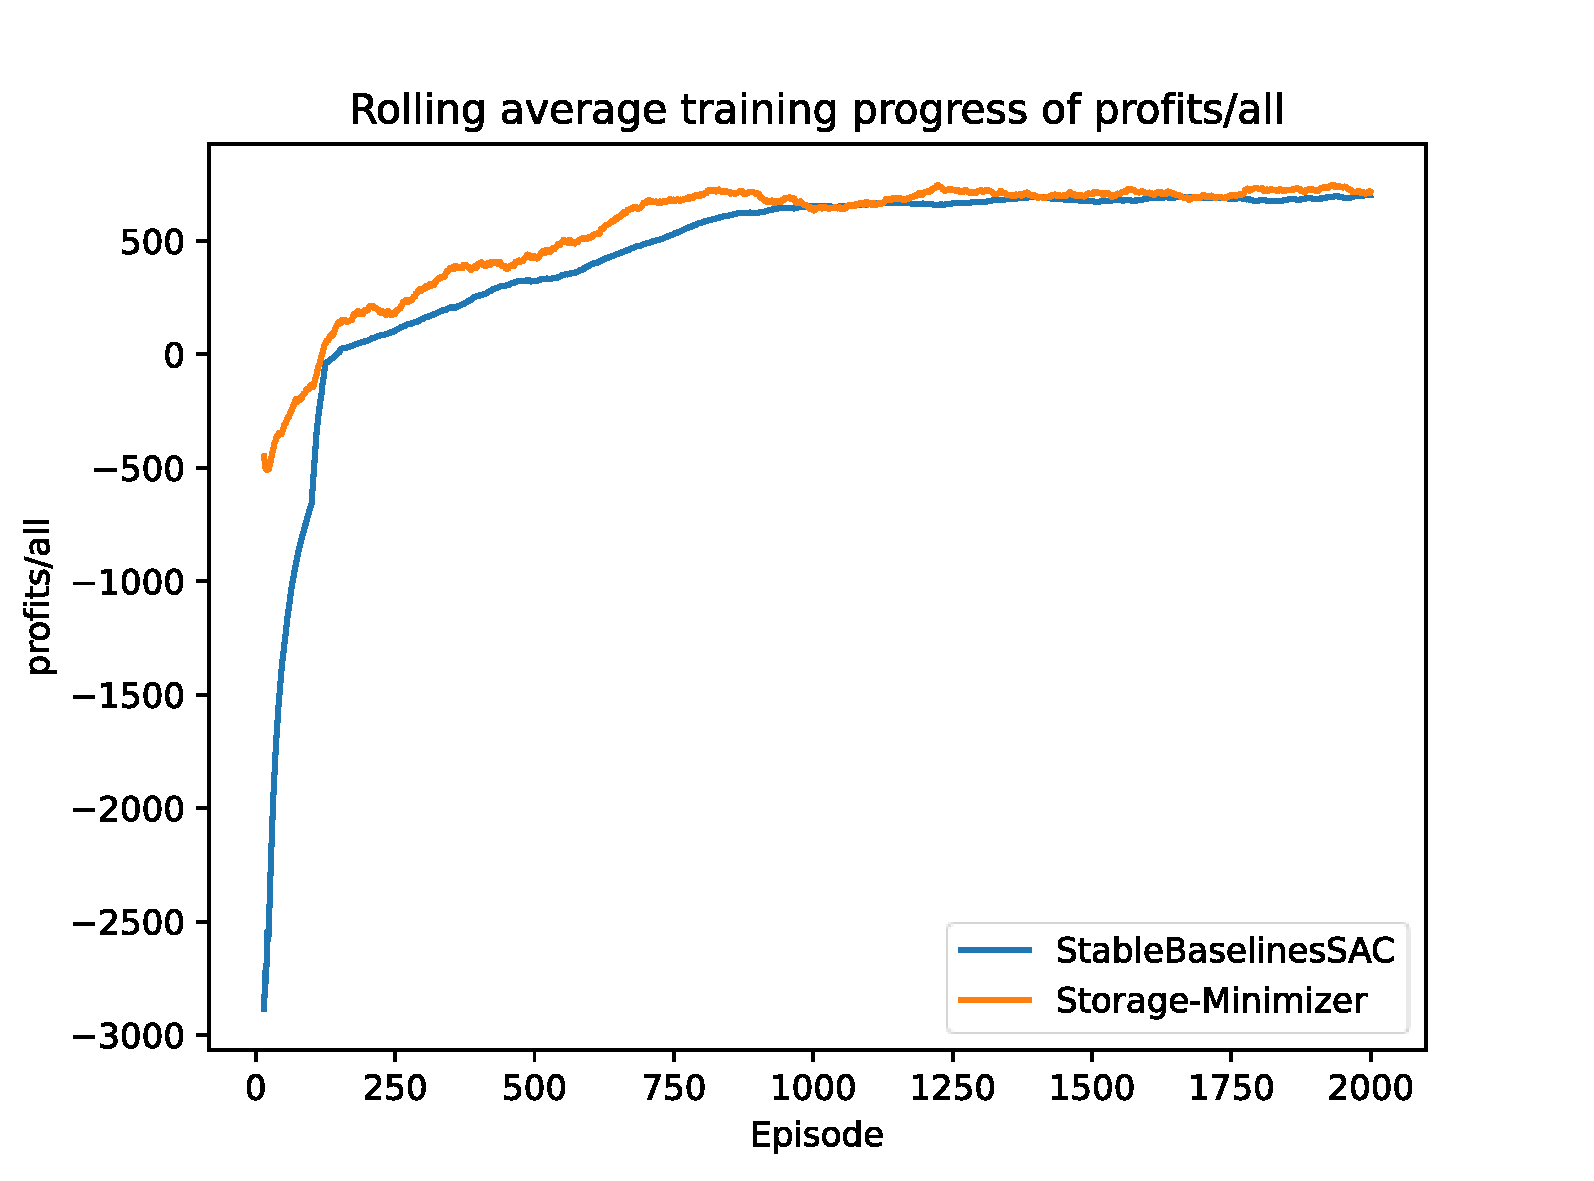
\includegraphics[width = .5\textwidth]{images/experiments/SACDuopoly/SACDuopolyProfits3.pdf}\\[1 ex]
	\end{subfigure}
	\caption{Profit per episode of three different training runs of an SAC-Agent on a Duopoly market}\label{fig:SACDuopolyProfits}
\end{figure}

\section*{Which graphs are how useful?}
\section*{What limitations are there?}
\section*{What can we do in the future to improve the graphs or the workflow?}
\section*{Can we see which hyperparameters influence the results in what ways using the diagrams?}
\section*{How can we improve the workflow (e.g. Grid-Search) with our analysis?}

